\chapter{Introduction}
\label{cha:introduction}

The work described in this dissertation is concerned with the implementation of a Java solution, named \texttt{xmlet}, that allows the automatic generation of a fluent \ac{API} based on a \ac{XSD} file. The generated classes are very similar most of the time and such solution may save time to the programmer, eliminating repetitive tasks and human error.

\section{Motivation}

Text has evolved with the advance of technology resulting in the creation of markup languages \cite{markuplanguages}. Markup languages work by adding annotations to text, the annotations being also known as tags, that allow to add additional information to the text. Each markup language has its own tags and each of those tags add a different meaning to the text encapsulated within them. In order to use markup languages the users can write the text and add all the tags manually, either by fully writing them or by using some kind of text helpers such as text editors with IntelliSense\footnote{\href{https://www.techopedia.com/definition/24580/intellisense}{Intellisense Definition}} which can help diminish the errors caused by manually writing the tags. But even with text helpers the resulting document can violate the restrictions of the respective markup language because the editors don't actually enforce the language rules. In the following \ac{HTML} example there is a violation of \ac{HTML} rules, a \texttt{<html>} tag containing a \texttt{<div>} tag, which is not allowed (Listing \ref{lst:failedhtml}).

\bigskip

\lstset{language=HTML}

\begin{lstlisting}[caption={Failed HTML rule validation},captionpos=b,label={lst:failedhtml}]
<html>
    <div>
        <!-- (...) -->
    </div>
</html>
\end{lstlisting}

\noindent
The solution to having documents that respect the markup language rules is changing the way the document writing works. As long as the writing process is fully controlled by the programmer errors will always happen because even though most text editors present the errors its corrections depend on the programmer correcting them. The suggestion presented is to move the writing control to an entity which can enforce the markup languages restrictions. This way it is guaranteed that the programmer won't be able to produce a document with errors. 

\noindent
Moving from the \ac{HTML} representation to a Java representation of the issue there are multiple solutions to solve it. In this first code sample the programmer is allowed to add any child to the \texttt{Html} element (Listing \ref{lst:runtimevalidationfailure}), resulting in a violation of the language restrictions, which is not detected unless the programmer verifies the result manually.

\bigskip

\lstset{language=Java, morekeywords={Html, Div}}

\begin{lstlisting}[caption={Lack of rule validation},captionpos=b,label={lst:runtimevalidationfailure}]
	Html root = new Html();
	root.add(new Div());
\end{lstlisting}

\noindent
To solve this problem the entity, \texttt{Html} class, should restrict the children and attributes that accepts based on the existing restrictions on the \ac{HTML}5 specification. As shown in the Figure \ref{motivation_2example} the generated \ac{API} enforces the language restrictions in compile time, this way guaranteeing that any document generated will be compliant with the respective specification.

\begin{figure}[h]
	\centering
	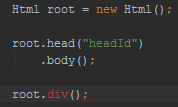
\includegraphics[width=0.4\textwidth]{motivation_2example}
	\caption{Error validation in compile time}
	\label{motivation_2example}
\end{figure}

\newpage

\noindent
This solution even though apparently solving the main problem introduces a new one. The new problem resides on the fact that manually recreating all the rules of a given markup language is normally a very long process since most markup languages have a vast number of elements, attributes and restrictions. 

\noindent
The solution for this new problem is automation. An automated process that converts the markup language definition of elements, its attributes and restrictions to classes that represent those elements and methods which enforce the specification rules. With this automated process the application can generate a fluent \ac{API} that allow the users to write their texts in a fluent way without errors and respecting the markup language specification. This is the main objective of this work, creating an infrastructure that reads a markup language definition, from a \ac{XSD} file, and generates an \ac{API} that allows the users to write well formed documents.

\section{Use case}
\label{sec:usecase}

The use case that will be used to test and evaluate the solution will be the \ac{HTML}5 \ac{XSD}. In this case there are multiple elements that share behavior and/or attributes that can be generated automatically. The generated classes allow to create a tree of elements that represent a \ac{XML} document. The resulting tree of elements can then be processed in different ways by using the Visitor pattern. This way each different Visitor implementation can use the generated tree of elements to write \ac{HTML} documents to a stream, a socket or a file. 

\noindent
The generated \ac{HTML}5 elements \ac{API} will then be used in the HtmlFlow \ac{API}, which is also a fluent Java \ac{API} that is used to write well formed \ac{HTML} files. With the Visitor pattern the HtmlFlow will only need to implement its own Visitor to achieve its goal. At the moment the HtmlFlow library only supports a set of the \ac{HTML} elements which were created manually and the rest of the library interacts with those elements in order to write the \ac{HTML} files. By using the solution which will be developed in this work the HtmlFlow will support the whole \ac{HTML} syntax. 

\section{Document Organization}

This document will be separated in five distinct chapters. The first chapter, this one, introduces the problem that was presented. The second chapter presents existent technology that is relevant to this solution. The third chapter explains in detail the different components of the suggested solution. The fourth chapter approaches the deployment and testing of the suggested solution. The fifth and last chapter of this document contains some final remarks and description of future work.